% Chapter Template

\chapter{Methodology} % Main chapter title

\label{Chapter4} % Change X to a consecutive number; for referencing this chapter elsewhere, use \ref{ChapterX}

\lhead{Chapter 4. \emph{Methodology}} % Change X to a consecutive number; this is for the header on each page - perhaps a shortened title

%----------------------------------------------------------------------------------------
%	SECTION 1
%----------------------------------------------------------------------------------------

\section{Study Area and Data Processing}

For this study, the test site chosen was Kharagpur, Salua its surrounding region in West Bengal, India. The site covers predominantly agricultural fields and forest cover along with some urban buildup. RISAT-1 data has been acquired on January 4, 2013 with a central latitude of 22.208289$\degree$N,central longitude of 87.414885$\degree$E and at incidence angle of 48.11354$\degree$. Using polSARpro and QGIS software this single look complex data was used to produce a geo-referenced primitive RGB output corresponding to the complex data and the four geo-referenced stokes parameter TIFF files. These four images were used to derive the features used to classify the area under study.
\begin{figure}[!htbp]
\centering
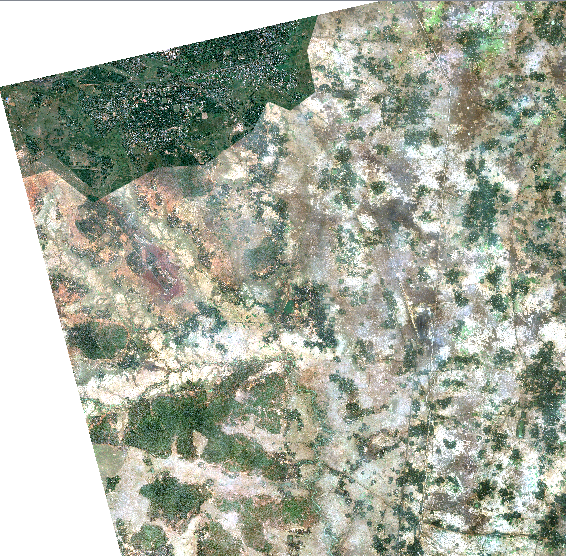
\includegraphics[width=50mm]{data1.png}
\caption{Google Earth image of the area under study. }
\label{fig2}
\end{figure}

Groundtruth for one-class SVM only contained reference pixels of forest cover in the whole area of study. Groundtruth was acquired from the past decade's topology charts from the Government of India. Total number of pixels in the image is 49,006,994. Total number of labelled pixels is 4,915,924, which is approximately 10$\%$ of the total pixels under study.

Groundtruth for maximum likelihood classifier required negative instances of forest cover, this was added manually by going through the Google Earth image and the RGB output image, which showed patterns, labelling agricultural, water bodies and urban buildup as the second class other than forest. We select the region of interest for the non-forest class using QGIS plugin tool. Number of pixels in this class was also fixed to be same as forest pixels.

\begin{figure}[!htbp]
\centering
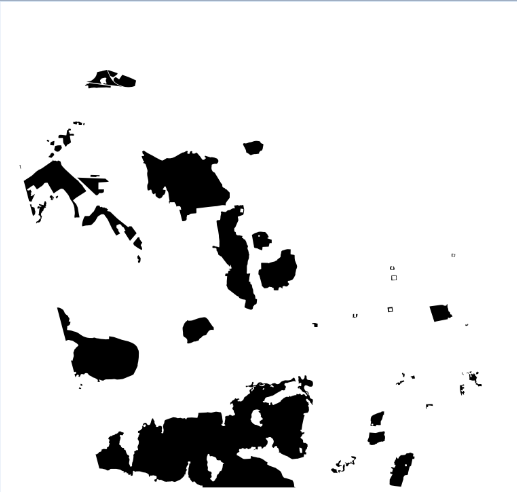
\includegraphics[width=60mm]{Pictures/data6.png}
\caption{Groundtruth showing black pixels as forest. }
\label{fig3}
\end{figure}

In case of maximum likelihood classifier, we require the groundtruth to be saved as spectral signature files, this is done using the QGIS software plugin tool. m-$\delta$ decompostion is done on the stokes parmaters images using the equations mentioned \ref{eq1} and \ref{eq2} we used our own python code to produce another image.  

\begin{figure}[!htbp]
\centering
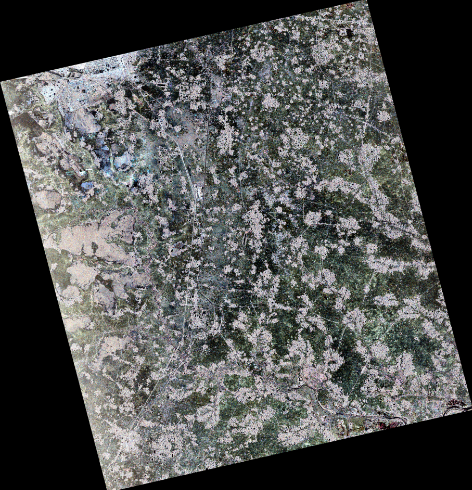
\includegraphics[width=60mm]{Pictures/data7.png}
\caption{RGB output image from polSARpro. }
\label{fig4}
\end{figure}


%----------------------------------------------------------------------------------------
%	SECTION 2
%----------------------------------------------------------------------------------------

\section{Image Classification}
We are trying to detect forest area in the dataset using two machine learning classification models, namely maximum likelihood classification and one class SVM. We will try to detect forest using two types of features, first the stokes parameter, secondly m-$\delta$ values. 

\subsection{Maximum Likelihood Classifier}

The classifier considers both the variances and covariances of the class signatures when assigning each cell to one of the classes represented in the signature file. A class can be characterized by the mean vector and the covariance matrix. Given these two characteristics for each pixel value, the statistical probability is computed for each class to determine the membership of the pixels to the class. Each pixel is assigned to the class to which it has the highest probability of being a member.

 The classifier we used in our work uses QGIS Semi-Automatic Classification Plugin Tool \cite{congedo2016semi}. When a maximum likelihood classification is performed, first the mean vector and covariance matrix is computed from the signature files given as groundtruth. Then the statistical probabilty is computed for each pixel in the whole image. We do this for both stokes paramters and m-$\delta$ value. In case of stokes paramter we add all four separate stokes parameter images as input to calculate the mean vector and covariance matrix. 
 
 We finally generate a TIFF file that is georeferenced to the location of the dataset and can then compare the results visually too in QGIS.


\subsection{One Class SVM}

We used the python interface for LIBSVM to implement the One Class SVM. The procedure that we followed :
\begin{itemize}
\item Transform the data to the format of the SVM package. 	 
\item Use cross-validation to find the best parameter  $\nu$ and $\gamma$.
\item Use the best parameter $\nu$ and $\gamma$ to train the whole training set.
\item Test on the whole dataset.
\end{itemize}
Before we train and test we have to decide on the size of the split of the complete ground truth; this needs to be done for various sizes to compare the accuracy.

\subsubsection{Training}\label{train}

We only have positive instances of the forest cover, inorder to train this we have to first create two vectors \textbf{X} (features or attributes) and \textbf{Y} (label). Each pixel in the training set has a value of +1 in \textbf{Y} and all four corresponding stokes parameter pixels(four dimensional) in \textbf{X} for classification with stokes parameters as feature, this changes to corresponding m-$\delta$ pixels (two dimensional) when we are classifying on the m-$\delta$ features. 

We then construct a problem in python format, This done using the svm\_problem() function predefined in the svmutil package. The parameters are set using the svm\_parameter() function, here we have to specify that our problem is a one-class SVM problem, uses an RBF kernel and set the value for the two parameters defined for the 
One class SVM namely $\nu$ (nu) and $\gamma$(gamma). After the problem is defined and the parameters are set, we can train and save the model for future use. Training typically takes 48 hours and we can save this time by saving the model when using the  same parameters and training set. 

\subsubsection{Testing}

In addition to testing on the test set we defined, we also have to test the data on the whole dataset to detect forest cover in unknown regions. Therefore, we have to have the whole dataset prepared in the same format discussed in \ref{train} as \textbf{Y} and \textbf{X}, for unknown pixels we denote values in \textbf{Y} as -1.
We use the svm\_predict() function to predict the label of the unknown pixel as either 1(for forest) or -1(for non-forest). After predicting for the entire dataset we create a final output image that can be viewed to assess the accuracy.

\subsubsection{Hyper-parameter tuning}

This is an important step in the classification using one class SVM. There are two parameters for an RBF kernel: $\nu$ and $\gamma$. It is not known beforehand
which $\nu$ and $\gamma$ are best for the given problem; consequently some kind of model selection (parameter search) must be done. The goal is to identify good ($\nu$ , $\gamma$) so that the classifier can accurately predict unknown data (i.e. testing data).

We try to find the best parameter pair using two techniques: grid-search and cross-validation.In n-fold cross-validation, we first divide the training set into n subsets of equal size. Sequentially one subset is tested using the classifier trained on the remaining n − 1 subsets. Thus, each instance of the whole training set is predicted once so the cross-validation accuracy is the percentage of data which are correctly classified \cite{hsu2003practical}.

Grid-search on $\nu$ and $\gamma$ using cross-validation is the recommended approach as in \cite{hsu2003practical}. Various pairs of ($\nu$ , $\gamma$) values are tried and the one with the best cross-validation accuracy is
picked. 



